\documentclass[a4paper,12pt,oneside]{book}
\author{Benjamin Uzan Muyumba}
\usepackage[french]{babel}
\usepackage[T1]{fontenc}
\usepackage[left=3.5cm,right=2cm,top=3.5cm,bottom=2cm]{geometry}
\usepackage[sorting=none]{biblatex}
\usepackage[acronym]{glossaries}
\usepackage{csquotes}
\usepackage{titlesec}
\usepackage{sectsty}
\usepackage{hyperref}
\usepackage{pifont}

\addto\captionsfrench{% Replace "english" with the language you use
  \renewcommand{\contentsname}%
    {TABLE DES MATIÈRES}%
}

\setcounter{secnumdepth}{4}
\setcounter{tocdepth}{4}

\chapterfont{\centering\large}
\sectionfont{\large}
\subsectionfont{\large}
\subsubsectionfont{\large\selectfont}

\addbibresource{main.bib}
\AtBeginDocument{\def\labelitemi{$\bullet$}}

\begin{document}
    \frontmatter
        \pagenumbering{Roman}
        \chapter*{ÉPIGRAPHE}
\addcontentsline{toc}{chapter}{ÉPIGRAPHE}
    \enquote{\it Le travail de management d’une clientèle est à la vente ce
    que, pour l’agriculture, le travail de fertilisation et
    d’entretien des sols est à la récolte.}
    \begin{flushright}
        \it - Pascal PY
    \end{flushright}

        \addcontentsline{toc}{chapter}{DÉDICACE}
\chapter*{DÉDICACE}
\thispagestyle{empty}
\clearpage
        \chapter*{REMERCIEMENTS}
\addcontentsline{toc}{chapter}{REMERCIEMENTS}
    Ce travail qui coiffe ainsi la fin de notre premier cycle est le
    résultat de multiples efforts tout au long de notre formation conformément
    au programme académique. Ce produit scientifique tel qu’élaboré ne présente
    en aucune manière le fruit de nos efforts personnels, elle est l’émanation
    des efforts conjugués de plusieurs personnes d’amour et de bonne volonté
    sans lesquelles il nous serait impossible de tous les représenter.
    \par
    C’est ainsi qu’au seuil de ce travail, de labeur, de persévérance,
    de courage qu’il soit permis d’adresser nos sincères et vifs remerciements 
    au professeur André LISONGOMI BATIBONDA pour ses conseils, sa disponibilité et pour avoir également accepté
    de diriger ce travail de main de maitre malgré ses multiples occupations.
    \par
    Nos remerciements s’adressent au corps administratif et professoral de l’école supérieure d’informatique
    Salama (ESIS) particulièrement à nos coordinateurs de filière madame Allegra NZEBA et monsieur Deoel MWANAKAHAMBO. %A REVOIR
    \par
    À tous les professeurs, intervenants et toutes les
    personnes qui par leurs paroles, leurs écrits, leurs conseils et leurs critiques ont guidé mes réflexions
    et ont accepté à me rencontrer et répondre à mes questions durant mes recherches. 
    \par
    À nos amis et collègues de la grande famille Génie Logiciel
    pour leur collaboration, leur solidarité et leur présence tout au long de notre
    parcours, dans les bons comme dans les mauvais moments.
    \par
    À l’Éternel Dieu Tout-Puissant pour tous ses bienfaits durant mon parcours.
    \par
    Trouvez ici nos sincères remerciements et que Dieu bénisse tous ceux qui m’ont aidé durant mes études supérieures et
    universitaires.
        \tableofcontents
\addcontentsline{toc}{chapter}{TABLE DES MATIÈRES} 

        \chapter*{AVANT-PROPOS}
\addcontentsline{toc}{chapter}{AVANT-PROPOS}
Ce travail portant sur \enquote{La conception d’un système informatisé de fidélisation
de la clientèle intégrant un système d’aide à la décision dans une entreprise de transport
de biens et de personnes} cas de la société TRANS NGOKAF.
\par
C’est dans le soucie de faciliter la fidélisation du segment client
dans la Gestion de la relation clients, que nous avons été inspire
à réaliser ce travail pour apporter un plus à la société TRANS NGOKAF
qui est notre cas d’étude et à toutes les entités qui détiennent des entreprises
de transport désireuses d’innovation et de rentabiliser le 
déluge d’information, de tirer profit de notre humble apport, fruit
de nos recherches et de nos expériences acquises dans le domaine informatique.
    \mainmatter
        \chapter*{INTRODUCTION GÉNÉRALE}
\addcontentsline{toc}{chapter}{INTRODUCTION GÉNÉRALE}
    %%%%%%%%%%%%%%%%%%%%%%%%%%%%%%%%%%%%%
    %% SECCTION A ABSOLUMENT SUPPRIMER %%
    %%%%%%%%%%%%%%%%%%%%%%%%%%%%%%%%%%%%%
    \section[Sujet]{Sujet}
    La présente étude porte sur la \enquote{Conception d’un système informatisé
    de fidélisation de la clientèle intégrant un système d’aide à la décision
    dans une entreprise de transport de biens et de personnes}.
    À ce sujet, nous avons pris le cas de la société de transport TRANS NGOKAF.
    
    \section[Contexte du sujet]{Contexte du sujet}
    La recherche scientifique anime aujourd’hui tout chercheur
    à pouvoir observer de manière
    plus particulière son environnement. Ce dernier étant
    sans cesse changeant, le chercheur se voit donc
    dans l’obligation de s’adapter aux différentes transformations
    survenant dans son environnement, ce qui n’est pas chose facile.
    Ainsi, suite à tous ces changements, le scientifique au cœur du
    développement rencontre plusieurs problèmes à résoudre en
    fonction de son domaine de recherche notamment, l’informatique,
    la médecine, l’architecture, l’économie, etc.
    \newline

    À l’exemple du domaine
    économique, la prise des décisions est devenue
    le point primordial pour une bonne gestion de
    l’entreprise. Une bonne décision engendre l’efficience,
    c’est-à-dire la réalisation des objectifs
    poursuivis tout en produisant une valeur ajoutée.
    \newline

    La plupart des entreprises du monde disposent d’une masse de données plus ou
    moins considérable. Ces informations proviennent soit de sources internes (générées par
    leurs systèmes opérationnels au fil des activités journalières), ou bien de sources externes
    (web, partenaire, etc.). Cette surabondance de données, et l’impossibilité des systèmes
    opérationnels de les exploiter à des fins d’analyse conduit, inévitablement, l’entreprise à se
    tourner vers un nouvel informatique dite décisionnelle qui met l’accent sur la
    compréhension de l’environnement de l’entreprise et l’exploitation de ces données à bon
    escient.
    \newline

    En effet, les décideurs de l’entreprise ont besoin d’avoir une meilleure vision de
    leur environnement et de son évolution, ainsi, que des informations auxquelles ils peuvent
    se fier. Cela ne peut se faire qu’en mettant en place des indicateurs de performance clairs
    et pertinents permettant la sauvegarde, l’utilisation de la mémoire de l’entreprise et offrant
    à ses décideurs la possibilité de se projeter et de se reporter à ces indicateurs pour une bonne
    prise de décision.
    \newline

    Ainsi toutes les entreprises commerciales partagent aussi
    le plus souvent un certain nombre de souhaits : gagner
    du temps, prendre du recul par rapport aux urgences, obtenir une meilleure
    stabilité de leurs recettes, mieux organiser leur travail et obtenir un meilleur
    revenu. \cite*{Barouch2010}
    \newline

    La rentabilité de la masse d’information (pouvoir transformer ce déluge
    d’information en valeur ajoutée), l’information étant un gage de compétitivité, surtout
    de nos jours, toute entreprise voulant prospérer se doit de prioriser la bonne gestion de
    cette dernière.

    \section[Problématique]{Problématique}
    La rédaction de tout travail scientifique implique au préalable une préoccupation.
    C’est dans le soucie de fidéliser le segment client de la société TRANS NGOKAF qui est une
    entreprise active dans le domaine du transport des biens et des personnes que nous
    réalisons ce travail.
    \newline
        
    De par le monde, les entreprises détenant une très grande part de marché
    se sentent le plus souvent à l’abri de toute concurrence
    dans leurs domaines d’activité grâce à la maitrise des rouages des affaires
    ou d’une quelconque technologie. \cite*{Rouviere2010} Et de ce fait
    certain d’entre elles ne s’occupent plus tant que ça de leurs relations clients.
    \newline

    C’est ainsi que nous prenons comme cas d’étude une des filiales de l’entreprise NGOKAF,
    qui exerce ses activités dans le domaine du transport de biens et de personnes, dénommée
    TRANS NGOKAF.
    \newline

    Notre étude se situe dans un environnement où la fidélisation n'est pas la principale
    préoccupation de l’entreprise, ce qui est une erreur, car c’est bien là la clé
    de la rentabilité et de la réussite de l’entreprise, car elle la rend plus performante.
    Pour cela nous essayerons d’articuler nos recherches autour des questions sui : 
    \newline

    Une question générale :
    \newline 
        \begin{itemize}
            \item [\ding{226}] Comment la société de transport TRANS NGOKAF gère-t-elle
            la relation client ?
            \newline
            \item [\ding{226}] Comment TRANS NGOKAF fait-elle pour fidéliser sa clientèle ?
            \newline
            \item [\ding{226}] Comment identifie-t-elle les clients pour une
            meilleure relation client ?
            \newline
            \item [\ding{226}] De quelle manière obtient-elle le retour client ?
        \end{itemize}
    \section[Hypothèses générales]{Hypothèses générales}
    Après avoir réalisés des recherches préliminaires, nous pouvons émettre, au regard
    de notre problématique, les hypothèses suivantes : 
    \newline
    \begin{itemize}
        \item [\ding{226}] Une application web sera réalisée, ce qui permettra de collecter
        les informations de la clientèle et leurs retours concernant les prestations de l’entreprise.
        \newline
        \item [\ding{226}] Afin d’effectuer du marketing ciblé sur les clients, un outil d’aide à
        la décision sera intégrer à l’application.
        \newline
        \item [\ding{226}] Un moyen de fidélisation par campagne promotionnelle sera réaliser.
        \newline
    \end{itemize}
    
    \section[Choix et interet du sujet]{Choix et intérêts du sujet}
        \subsection[Choix du sujet]{\textit{Choix du sujet}}
        Dans le cadre général, le choix porté sur ce sujet a été motivé par le souci d’aider
        la société TRANS NGOKAF de pouvoir fidéliser plus aisément le segment client à laide d’un
        système intégrant un système d’aide à la décision.
        \subsection[Interet du sujet]{\textit{Intérêts du sujet}}
        L’intérêt du sujet se réfère à l’importance et à la pertinence du sujet choisi pour notre recherche.
        Un sujet intéressant est celui qui est pertinent pour les autres parties impliquées dans nos recherches.
        Il doit être capable de susciter l’intérêt et de motiver les recherches et la rédaction. C’est ainsi
        que nous nous en retiendrons trois :
         \newline 
            \begin{itemize}
                \item [\ding{226}] Intérêt personnel : en tant qu’ingénieur en management 
                des systèmes d’information, nous serons heureux d’apporter une solution
                qui aidera les entreprises de transport de biens et de personnes de fidéliser
                le segment client.
                \newline

                \item [\ding{226}] Intérêt sociétal : la réalisation de ce système
                informatisé de fidélisation de la clientèle permettra à TRANS NGOKAF
                de conserver sa part de marché actuel tout en la développant. 
                %%%%%%%%%%%%%%%%%%%%%%%%%%%%%%%%%%%%%%%%%%%
                %% SOLUTION POUR LES GENERATIONS FUTURES %%
                %%%%%%%%%%%%%%%%%%%%%%%%%%%%%%%%%%%%%%%%%%%
                %% et dans le meilleur des cas mettre en place une stratégie
                %% de prospection pour accroitre sa clientèle.
                Selon Bain \& Cie : \enquote{\textit{5 \% d’augmentation du taux de
                rétention sur les meilleurs clients peut générer entre 25 et 55 \%
                d’augmentation des bénéfices d’une entreprise.}} \cite*{Siecdigi}
                \newline

                \item [\ding{226}] Intérêt scientifique : dans le système LMD
                \footnote[1]{LMD : Licence-Master-Doctorat} tout étudiant
                a le devoir, à la fin de son cycle d’étude, d’élaborer un travail qui
                sanctionne son parcours. Le bien fonder du travail de fin de cycle
                est de donner l’occasion à l’étudiant de prouver la maitrise et la bonne acquisition
                des notions apprises tout au long de son parcours dans une filière données.
            \end{itemize}
    \section[Démarches méthodologiques]{Démarches méthodologiques}
        \subsection[Méthodes]{\textit{Méthodes}}
        Une méthode est une manière de conduire sa pensée, d’établir ou de démontrer une
        vérité suivant certains principes et avec un certain ordre.
        \newline

        Dans le cadre de notre travail, nous utiliserons la méthode UP (Unified Process).
        Le Processus Unifié est un processus de développement logiciel \enquote{itératif et incrémental,
        centré sur l’architecture, conduit par les cas d’utilisation et piloté par les risques.} \cite{Roques2008}
        \newline

        UML se définit comme un langage de modélisation graphique et textuel destiné à
        comprendre et décrire des besoins, spécifier et documenter des systèmes, esquisser des
        architectures logicielles, concevoir des solutions et communiquer des points de vue. \cite{RoqVall2007}
        \newline
        
        UML est le moyen graphique de garantir que \enquote{ce qui se conçoit et se programme
        bien s’énonce clairement.\footnote[2]{Hugues \textsc{Bersisni}, \textit{La programmation orientée objet}, 7e édition, Eyrolles, Paris, 2017, p. 222}}
        \subsection[Techniques]{\textit{Techniques}}
        Les techniques sont des mécanismes qui nous permettent de réaliser nos recherches
        scientifiques. Pour rendre notre travail facile à réaliser nous avons pris comme techniques : 
        \newline
        \begin{itemize}
            \item [\ding{226}] L’interview : pour comprendre de façon simple notre travail, nous avons fait des
            descentes sur terrains, nous avons eu à interroger les techniciens et le manager
            informatiques, les professeurs informatiques, les collègues, les ainés scientifiques
            et ceux qui s’intéressent beaucoup plus à l’outil informatique.
            \newline
            \item [\ding{226}] L’observation : nous nous sommes données beaucoup du temps à observer plus
            attentivement, pour comprendre de manière précise comment ça se passe exactement sur un ordinateur fonctionnel.
            \newline
            \item [\ding{226}] La documentation : la lecture est le moyen efficace de voyager dans le monde
            de la connaissance. Comme un chercheur, pour parvenir à résoudre un problème
            dans la société, il nous faut une lecture consistante. Nous avons eu à utiliser les
            livres scientifiques, nous nous sommes rendus dans les bibliothèques, nous avons
            consulté des documents sur l’internet, nous avons utilisé différents médias afin de
            réunir toutes les informations dont nous avons besoin.
        \end{itemize}
    \section[Etat de l'art]{État de l’art}
    Ce travail se basant sur des informations et une structure d’entreprise particulière, nous ne
    pouvons pas déclarer que ce dernier est une recherche originale, car d’autre chercheur ont eu
    à traiter du sujet relativement similaire à celui-ci.
    \newline

    Nous avons notamment BUYAMABA SUZE Ange, dans le cadre de son travail de fin de cycle
    qui parlait de : \enquote{MISE EN PLACE D’UN SYSTÈME INFORMATISE DE FIDÉLISATION DES CLIENTS BASE SUR LES
    DONNÉES D’UN SERVICE TRAITEUR}. Ce travail base sur la conception d’un système informatisé de fidélisation des clients
    à aider la maison Excellence d’obtenir les retours clients dans la perspective d’une amélioration des services. \cite{Buyamba2017}
    \newline

    Cependant, il est impossible à la maison Excellence de savoir, grâce à des analyses et des visualisations, qui
    sont les meilleurs clients. Et sans oublier que sa recherche était concentré sur les services traiteurs. 
    \newline

    Mais en ce qui nous concerne nous rejoignions le chercheur cité ci-haut, dans le sens où nous traitons de manière
    générale d’une application de fidélisation, mais intégrant un système d’aide à la décision.
    % Divergence et conc=vergence -- demarcation
    \section[Délimitation du travail]{Délimitation du travail}
        Nos recherches ont été effectuer chez TRANS NGOKAF qui est une entreprise de transport
        située dans la ville de Lubumbashi, dans la province du Haut-Katanga en République Démocratique du Congo.
        \newline
        Notre Travail couvrira l’année 2023.
    \section[Subdivision du travail]{Subdivision du travail}
    Outre l’introduction générale et la conclusion générale, notre travail est subdivisé
    en trois chapitres :
    \newline
        \begin{itemize}
            \item [\ding{226}] Le premier chapitre : \enquote{cadre conceptuel et théorique}, présente une vue
            d’ensembles des concepts de base du sujet et quelques théories sur la méthodologie
            utilisée du travail.
            \newline
            \item [\ding{226}] Le deuxième chapitre : \enquote{analyse conceptuelle du système d’information}, 
            décrit l’analyse de l’architecture métier dans lequel nous allons présenter un système existant
            et le processus de l’organisation du travail ainsi que le futur système.
            \newline       
            \item [\ding{226}] Le troisième chapitre : \enquote{analyse et conception du système}, s’appuie sur la
            modélisation de notre système métier et est basé sur l’explication de différentes
            technologies utilisées pour l’implémentation ou développement de notre solution.            
        \end{itemize} 
    \section[Outils logiciels et équipements utilisés]{Outils logiciels et équipements utilisés}
    %%%%%%%%%%%%%
    %% A VENIR %%
    %%%%%%%%%%%%%
    Après avoir présenté le contexte et les enjeux de notre recherche, nous allons maintenant nous pencher sur
    les différents concepts, théories et méthodes utilisées.
        \chapter[CADRE CONCEPTUEL ET THÉORIQUE]{CADRE CONCEPTUEL ET THÉORIQUE}

        \chapter[ANALYSE CONCEPTUELLE DU SYSTÈME D’INFORMATION]{ANALYSE CONCEPTUELLE DU SYSTÈME D’INFORMATION}
    \section[Introduction partielle]{Introduction partielle}
    Dans ce chapitre, nous allons présenter l’environnement professionnel dans lequel notre
    travail se déroule.
    \par
    Premièrement nous commençons d’abord par une brève présentation de Ngokaf Trans, puis nous introduisons
    la structure générale de son organisation avec ses différentes directions en particulier
    sa direction marketing pour qui notre projet est destiné, nous détaillons son organigramme ainsi
    que ses objectifs. 
    \par
    Et deuxièmement nous faisons une description du système d’information existant ainsi
    que du futur système d’information en ressortissant les besoins fonctionnels et non
    fonctionnels de ce dernier.
    \section[Environnement de travail]{Environnement de travail}
        \subsection[Présentation]{\textit{Présentation}}
        La société Ngokaf Trans est une compagnie de transport routier
        par bus de biens et de personnes, en République Démocratique du Congo
        et particulièrement dans les provinces du Haut-Katanga et du Lualaba.

        \subsection[Aperçu historique]{\textit{Aperçu historique}}
        La société Ngokaf Trans a été créée par Monsieur NGOIE KAFULA Didas,
        elle débute ses activités en 2020 dans le
        souci de rendre facile les déplacements de la population dans des conditions confortable
        dans les villes du sud de la République Démocratique du Congo.
        Rapidement la compagnie se développe et effectue des trajets, au départ
        entre Lubumbashi et Likasi, aujourd’hui entre Lubumbashi
        et Kolwezi. 

        \subsection[Situation géographique]{Situation géographique}
        Son siège social, se situe dans la province du Haut-Katanga, dans la ville de Lubumbashi,
        dans la commune de Lubumbashi sur croisement des avenues Moero et Kapenda.        

        \subsection[Objectifs sociaux]{Objectifs sociaux}
        La société Ngokaf Trans \acrshort{sarl} est une société commerciale,
        dont l’activité principale est :
        \par
        \begin{itemize}
            \setlength{\itemsep}{0pt}
            \item [\ding{226}] Le transport des personnes et des biens entres les différentes villes.
            \item [\ding{226}] Offrir les meilleurs services aux clients.
            \item [\ding{226}] Offrir des tarifs à bas prix permettent aux clients de voyager à travers les villes.
        \end{itemize}
        \subsection[Structure Organisationnelle]{Structure Organisationnelle}
            \subsubsection[Le Directeur Général]{Le Directeur Général}
            Le Directeur Générale planifie, dirige et supervise les activités reliées
            au transport, aux études d’élargissement, au rayonnement interne et externe
            de l’agence ainsi qu’à l’administration générale de la société.
            \par\noindent
            Le Directeur Générale de Ngokaf Trans s’assure également que les valeurs
            institutionnelles et les exigences de performances au sein de l’entreprise sont respectées.

            \subsubsection[Le Manager]{Le Manager}
            Le Manager est le représentant numéro 1 du Directeur vu que celui-ci ne vit pas au pays,
            il a le rôle d’anticiper les risques, les tendances et les opportunités ; c’est lui décide
            et fait les choix stratégiques et tactiques. C’est lui qui recadre évalue les agents ;
            il a en même temps de rôle d’écouter, rédiger et présenter les feeds-back.
            Les problèmes cruciaux au sein de Ngokaf Trans sont résolus par le Manager,
            la fonction de fédérer et motiver et superviser toutes les agences lui reviennent.

            \subsubsection[Le Secrétaire de Direction]{Le Secrétaire de Direction}
            Le secrétariat de direction chez Ngokaf Trans est un bureau stratégique
            qui collabore directement avec le Manager il joue un rôle fondamental dans
            la bonne marche.
            \par\noindent
            Les compétences techniques du secrétariat de Direction chez Ngokaf Trans
            lui permettent d’organiser et d’encadrer le travail administratif dont il a la charge.

            \subsubsection[Le Responsable des Ressources Humaines]{Le Responsable des Ressources Humaines}
            Il a comme mission :
            \par
                \begin{itemize}
                    \setlength{\itemsep}{0pt}
                    \item [\ding{226}] Établir et contrôler les paies spécifiques ;
                    \item [\ding{226}] Tenir à jour les dossiers du personnel et remplir les obligations légales ;
                    \item [\ding{226}] Organiser les élections des instances représentatives du personnel ;
                    \item [\ding{226}] Recruteur et intégrer le personnel.
                \end{itemize}
            \subsubsection[Le Contrôleur de Gestion]{Le Contrôleur de Gestion}
            Il a comme mission :
            \par
                \begin{itemize}
                    \setlength{\itemsep}{0pt}
                    \item [\ding{226}] Établir les prévisions d’activité en terme d’objectifs de budgets,
                    d’organisation et de moyen ;
                    \item [\ding{226}] Élaborer et adapter les outils d’analyse, les indicateurs et
                    procédures du contrôle de gestion ;
                    \item [\ding{226}] Identifier les écarts significatifs entre les réalisations et les prévisions ;
                    \item [\ding{226}] Mesure et analyser les écarts sous forme de statistiques, de tableaux de bord commentés et de rapport d’activités ;
                    \item [\ding{226}] Assurer la retransmission commentée des informations auprès de la direction générale.
                \end{itemize} 
            \subsubsection[Le Responsable Financier]{Le Responsable Financier}
            Il a comme mission :
            \par
                \begin{itemize}
                    \setlength{\itemsep}{0pt}
                    \item [\ding{226}] Contrôler la comptabilité de l’entreprise et la bonne
                    gestion de sa trésorerie, soit valider la rentabilité de l’entreprise ;
                    \item [\ding{226}] Développer des outils d’aide à la prise de décision ;
                    \item [\ding{226}] Valider la solvabilité de l’entreprise ;
                    \item [\ding{226}] Anticiper la stratégie de développement de l’entreprise
                    et les différents investissements et financement nécessaires.
                \end{itemize}
            \subsubsection[Le Responsable Informatique]{Le Responsable Informatique}
            Il a comme mission :
            \par
                \begin{itemize}
                    \setlength{\itemsep}{0pt}
                    \item [\ding{226}] Assure la disponibilité des différents équipements ;
                    \item [\ding{226}] Superviser l’achat des équipements informatiques ;
                \end{itemize}
        \subsection[Organigramme de l’entreprise]{Organigramme de l’entreprise}
            \begin{figure}[h!]
                \centering
                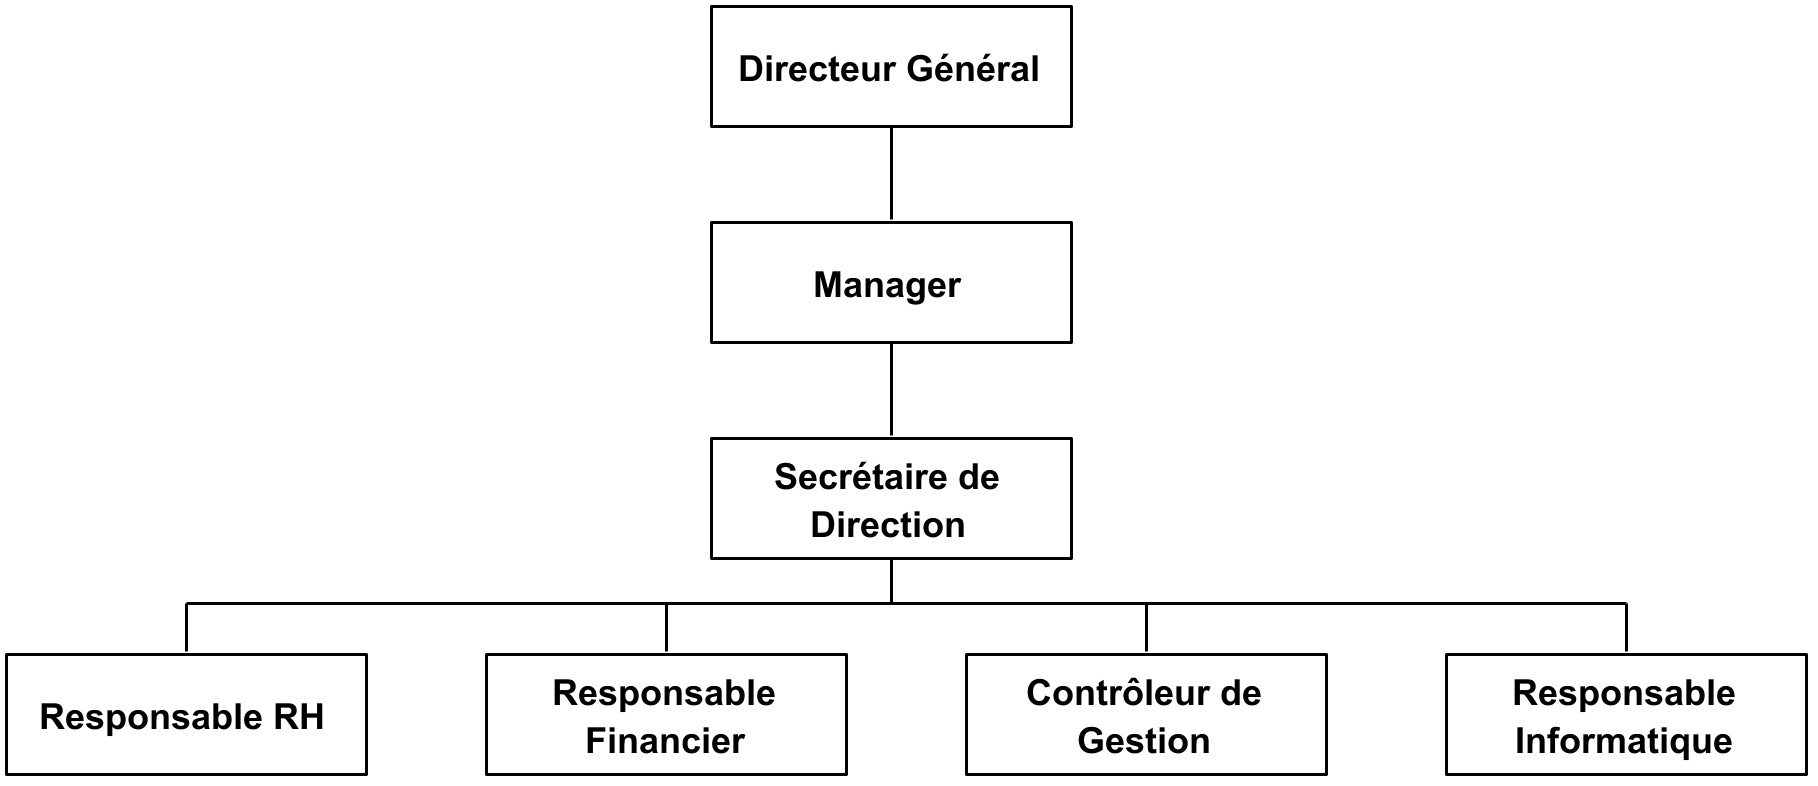
\includegraphics[width=140mm]{organigramme.png}
                \caption{Organigramme de la société Ngokaf Trans}
                \label{fig:Organigramme}
            \end{figure}
    \section[Analyse du système existant]{Analyse du système existant}
        \subsection[Procédures de ventes des billets]{Procédures de ventes des billets}
        Cette étape s’effectue comme suit :
\pagebreak
        \subsection[Diagramme d’activité métier]{Diagramme d’activité métier}
            \begin{figure}[h!]
                \centering
                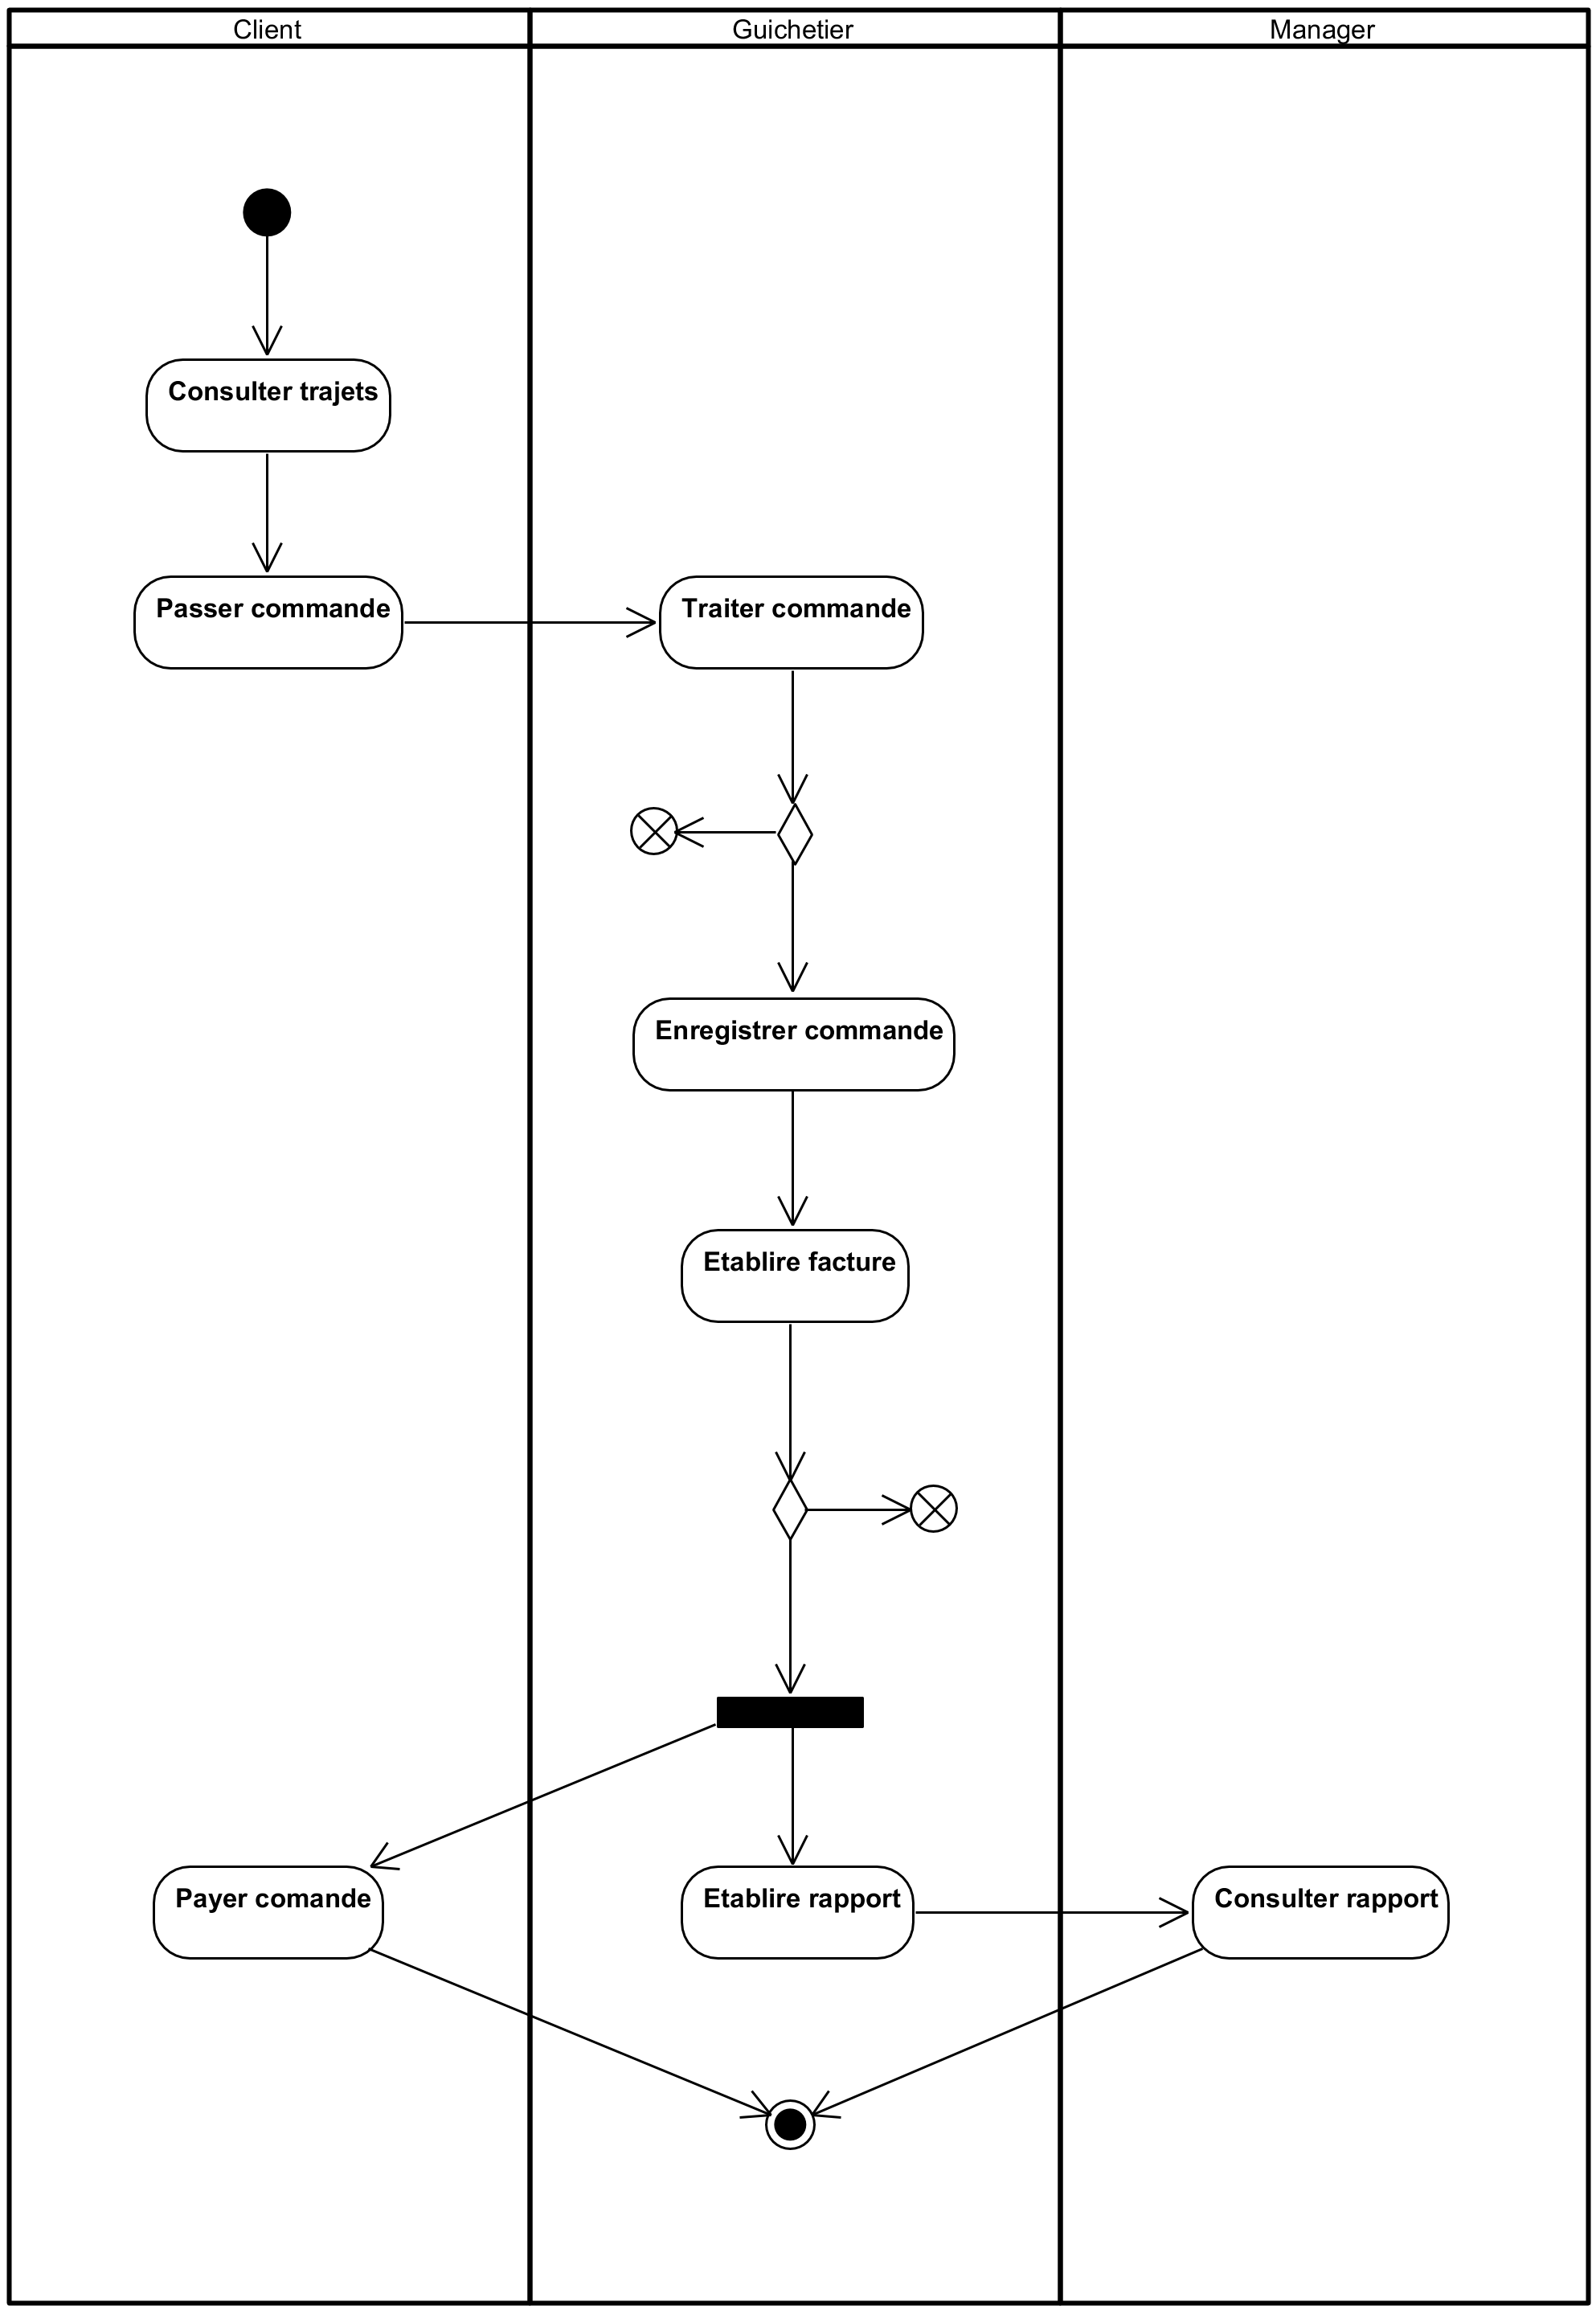
\includegraphics[width=140mm]{dac-metier.png}
                \caption{Diagramme d’activités métier}
                \label{fig:DacMetier}
            \end{figure}
\pagebreak
        \subsection[Système de fidélisation existant]{Système de fidélisation existant}
        L’entreprise Ngokaf Trans ne dispose d’aucun système de fidélisation de la clientèle
        par conséquent 
        \subsection[Système de prise de décision existant]{Système de prise de décision existant}
    \section[Critique du système existant]{Critique du système existant}
    Le point de départ de la récolte des données concernant le client étant le
    point de ventes des tickets de bus, 
    \section[Futur système]{Futur système}
    L’identification des besoins constitue la phase de départ de toute
    application à développer dans laquelle nous allons identifier
    les besoins de notre application. Nous distinguons des besoins
    fonctionnels qui présentent les fonctionnalités attendues de notre
    application et les besoins non fonctionnels pour éviter le développement
    d’une application non satisfaisante ainsi de trouver un
    accord commun entre les spécialistes et les utilisateurs pour réussir le projet.
        \subsection{Besoins fonctionnels}
        Les besoins fonctionnels décrivent les exigences fonctionnelles
        des différents acteurs de l’application.
        \subsection{Besoins non fonctionnels}
        Les besoins non fonctionnels sont les besoins qui ne sont pas des
        services rendus par le système, mais qui complètent les
        exigences fonctionnelles pour que la solution corresponde vraiment
        aux besoins des utilisateurs.
    \section[Conclusion partielle]{Conclusion partielle}
    Dans ce chapitre, nous avons procédé à la présentation de notre
    cadre de recherche qui est la société Ngokaf Trans. Nous avons étudié
    en détail le déroulement du processus, déniché les failles et les
    insuffisances dans le but de comprendre les problèmes rencontrés par la
    société Ngokaf Trans. Par la suite, nous avons identifié les besoins du
    point de vue de l’utilisateur qui est la société Ngokaf Trans, ainsi que
    les candidats, du point de vue technique en donnant une liste des exigences.
    \par
    Sur base de nos analyses, nous avons proposé une gestion de la clientèle et
    un système de prise de décision, concernant la fidélisation de la clientèle
    à l’aide d’une application informatisée. La connaissance de toutes les
    informations de notre analyse nous permettra dans le deuxième chapitre
    de modéliser le nouveau système proposer.
    \backmatter
        \appendix
        \printbibliography[heading=bibintoc,title={RÉFÉRENCES}]
\end{document}
